\documentclass{beamer}
\usepackage{amsmath}
% Required package
\usepackage{subcaption}
% so that the captions are numerated
\setbeamertemplate{caption}[numbered]
\usetheme{Frankfurt}
\newcommand\myfontsize{\fontsize{14pt}{18pt}\selectfont}

\usepackage{wrapfig}

\logo{

\includegraphics[width=1cm]{imsp_logo.jpeg}
}

\title{ Projet IoT: Utilisation du capteur d'humidité du sol \\ {\small IMSP Dangbo} }
\author{{\small \underline{Professeur} :} \textbf{Probus KIKI} \\ {\small \underline{Groupe 6} :} \textbf{Abel KPOHINTO} \& \textbf{Bénédite LOVI}}
\date{\today}

\begin{document}
	
	\frame{\titlepage}
	\begin{frame}{Sommaire}
    		\tableofcontents
	\end{frame}
	
	\section{ Introduction }
	\begin{frame}{\textbf{INTRODUCTION}}
	\begin{wrapfigure}{r}{0.5\textwidth}
    \centering
    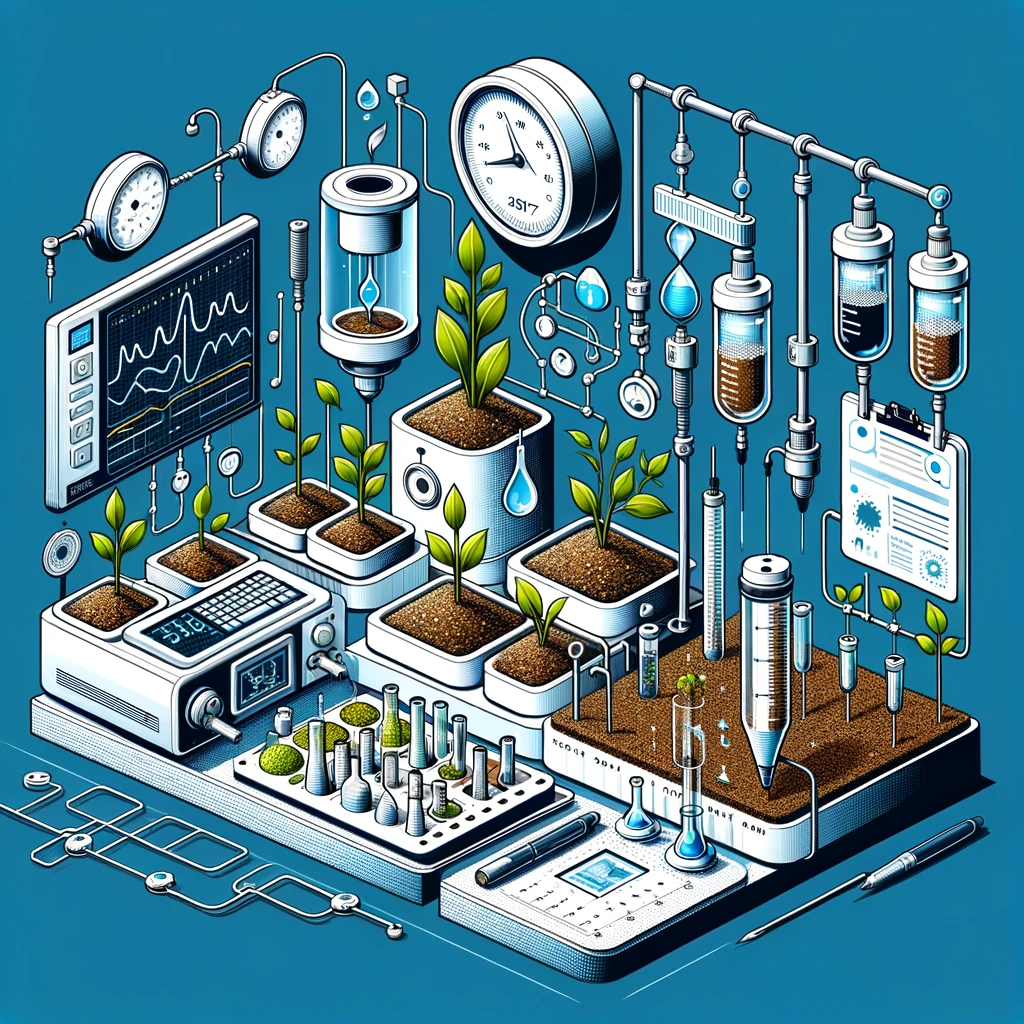
\includegraphics[width=0.7\textwidth]{intro.png}
    %\caption{Wrapping text around figures}
	\end{wrapfigure}

        L'utilisation des capteurs d'humidité du sol révolutionne de nombreux secteurs, allant de l'agriculture à la gestion environnementale et urbaine. Connectés à des microcontrôleurs tels qu'Arduino ou Raspberry Pi, ils permettent une surveillance précise et une meilleure gestion des ressources en eau, contribuant ainsi efficacement au développement durable dans divers domaines.

	\end{frame}
	\section{Présentation du projet}
	\subsection{Présentation du capteur d'humidité funduino}
	\begin{frame}{Présentation du capteur d'humidité funduino}
		Le capteur d'humidité du sol est constitué de deux parties principales : les sondes qui sont insérées dans le sol et le module électronique qui mesure la résistance électrique entre les sondes. La résistance varie en fonction du taux d'humidité du sol. Plus le sol est humide, plus la résistance est faible, et vice versa.
		\centering
    			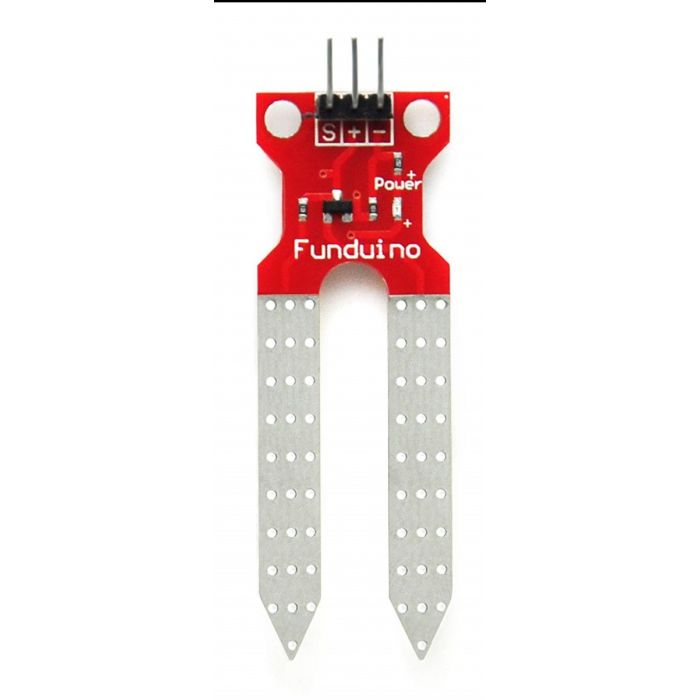
\includegraphics[width=5cm]{hum.jpg}
	\end{frame}
	\subsection{Présentation du cablage}
	\begin{frame}{Présentation du cablage}
		\centering
    			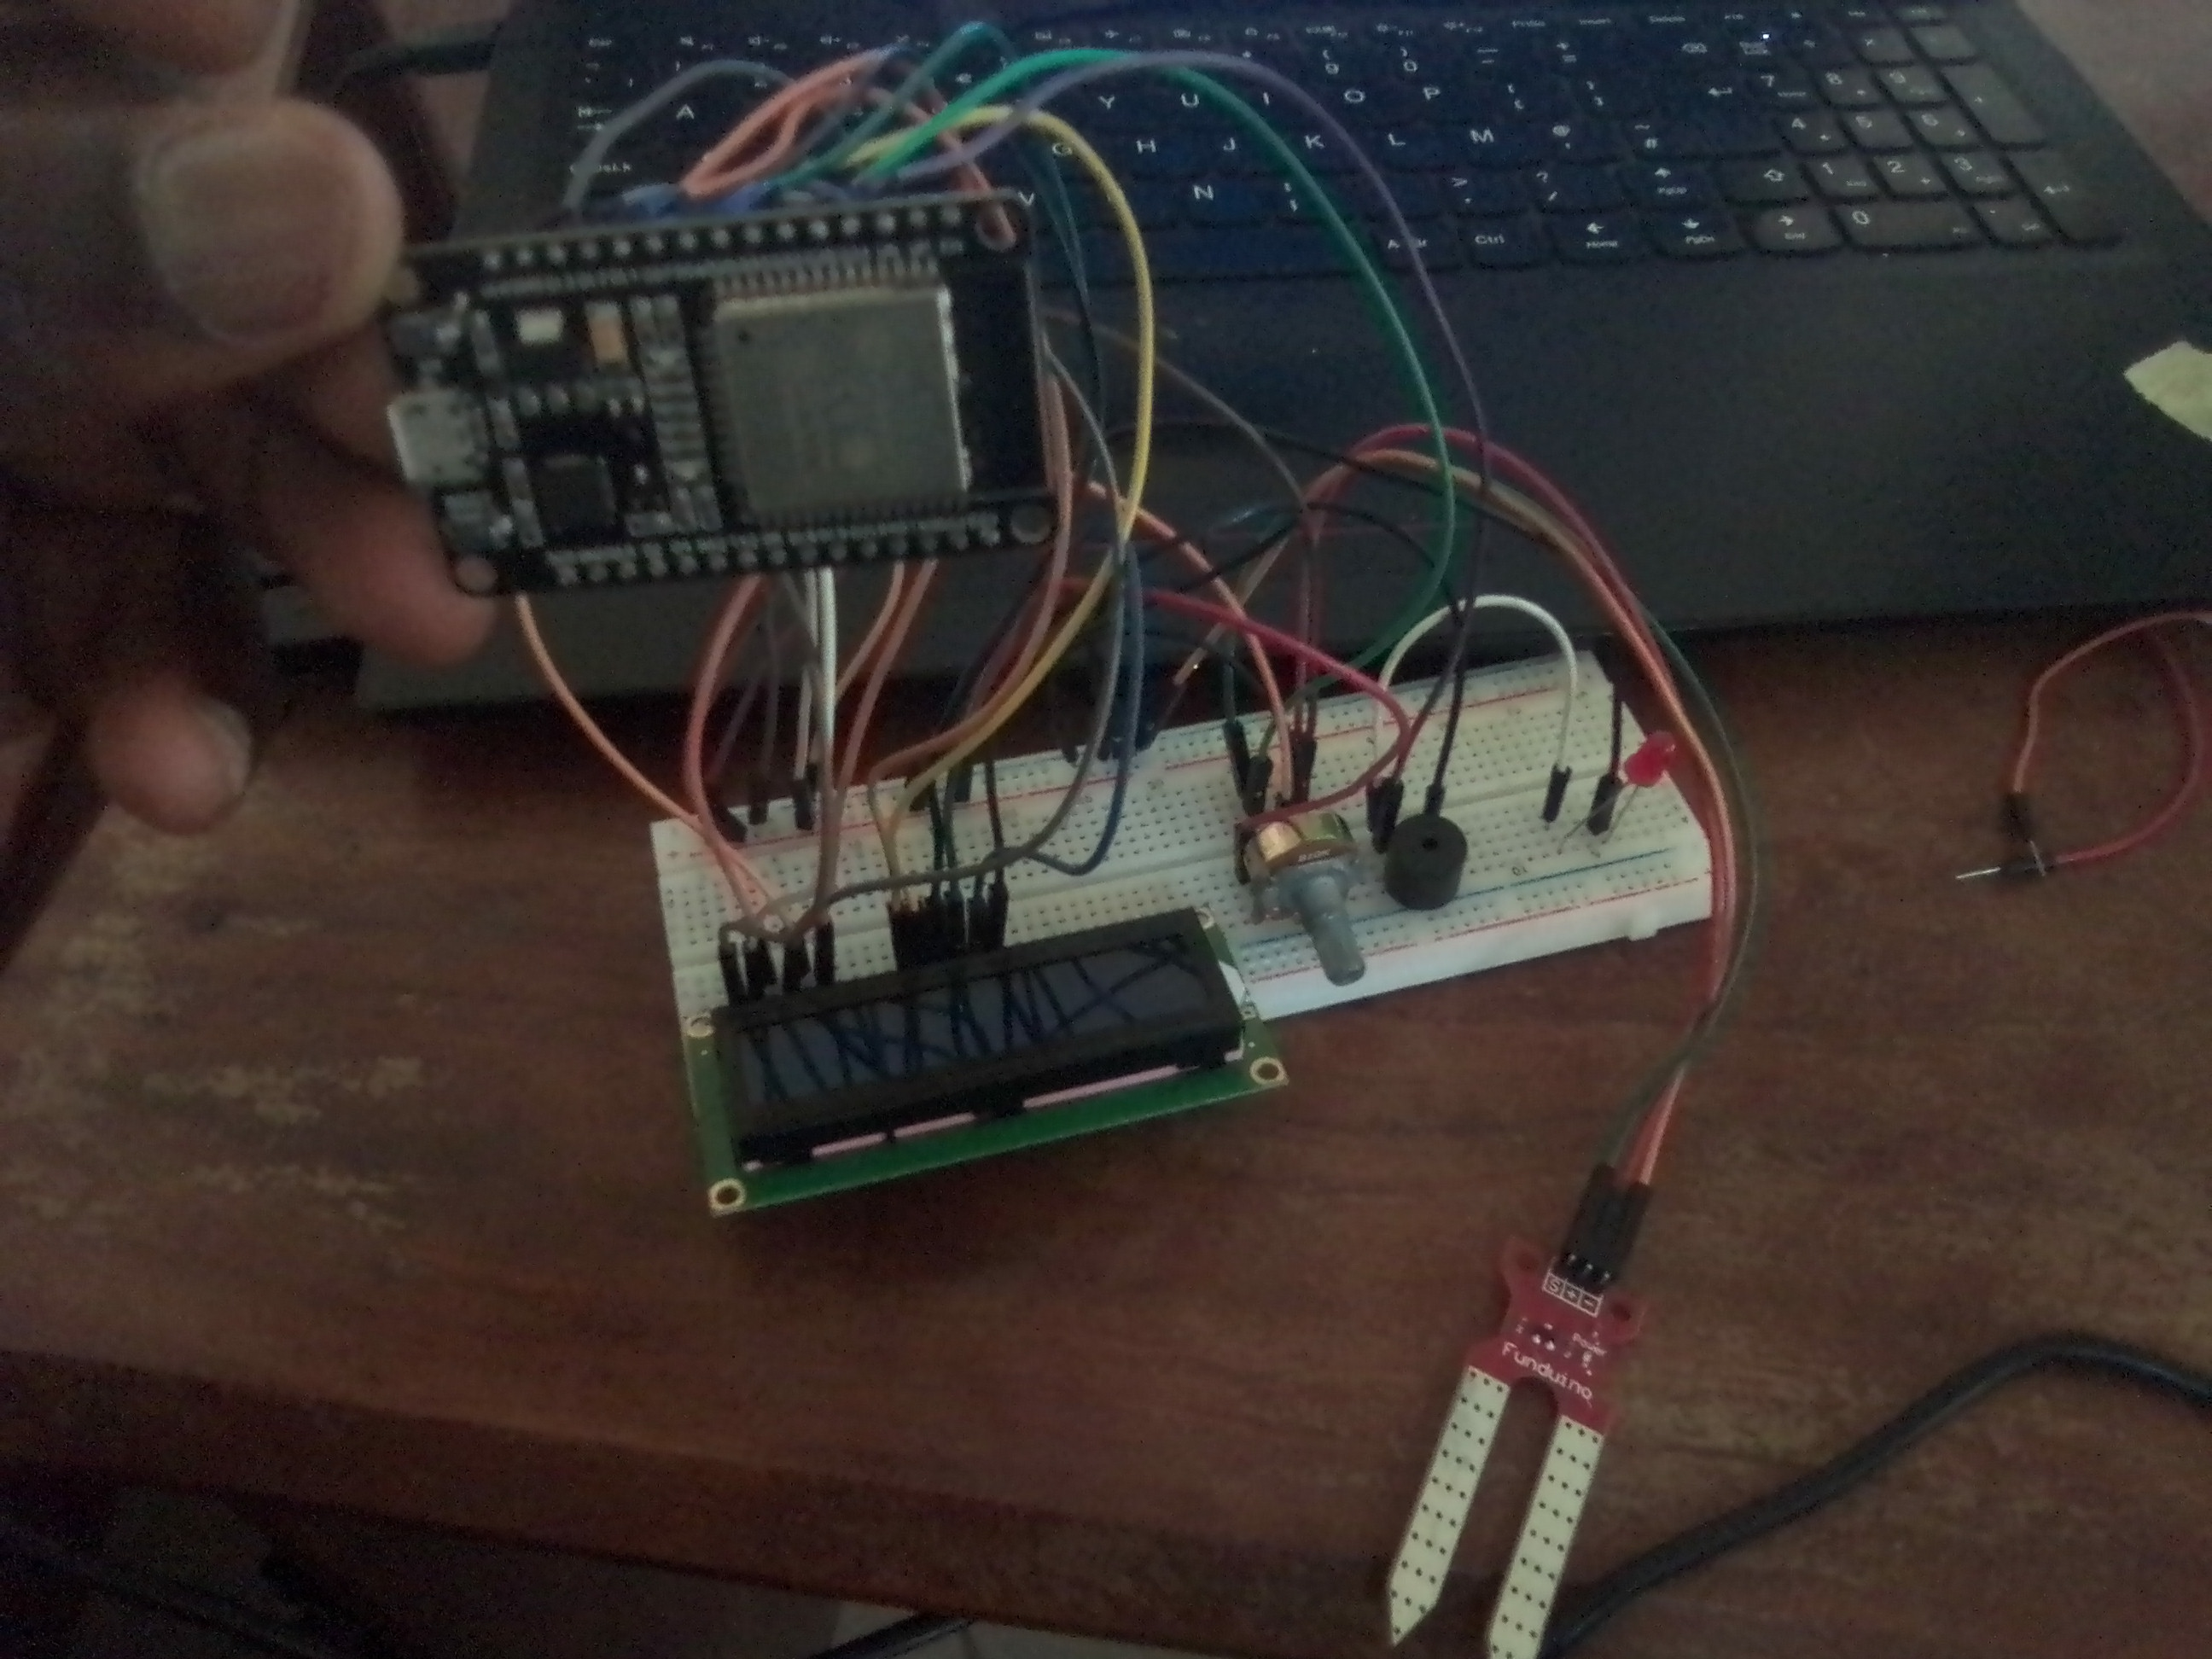
\includegraphics[width=10cm]{cablage.jpg}
	\end{frame}
	\subsection{Demo}
	\begin{frame}{Demo}
		\centering
		{\myfontsize \textcolor{blue}{\textbf{DEMO}}}
	\end{frame}
	\section{Conclusion}
	\begin{frame}{CONCLUSION}
		En résumé, les capteurs d'humidité du sol sont devenus un outil essentiel dans divers domaines, bien au-delà de l'agriculture. Leur utilisation soulève cependant une question pertinente pour la recherche future : comment pouvons-nous développer davantage ces technologies pour maximiser leur efficacité et étendre leurs applications à d'autres domaines critiques pour notre environnement et notre société ?"
	\end{frame}
	\begin{frame}
		\centering
		
\includegraphics[width=7cm]{thanks.jpg}
	\end{frame}
\end{document}
